\section{Real life examples}
\begin{example}
You are required to design an open box with a square base and a total volume of $4\mbox{m}^3$ using the least amount of materials.

We are hunting for particular dimensions of the box. Lets give them names, so we will call the length of the base edges $a$ and let the height of the box be called $b$.

\begin{figure}[H]
\centering
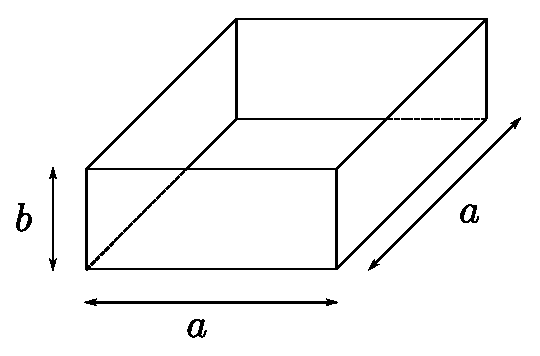
\includegraphics[scale=0.7]{img/real-life-box}
\caption{Square based open top box.}
\label{fig:real-life-box}
\end{figure}

In terms of $a$ and $b$, the volume of the box is 
\[a^2b=4 \mbox{ (m}^3\mbox{)}. \]

We want to minimise the amount of material, so we must look at how much material is used. We have a base of area $a^2$ and 4 sides, each with area $ab$. So the total area is
\[a^2+4ab.\]

We want to find the minimum value of $a^2+4ab$, subject to the condition $a^2b=4$ and more obviously $a>0$, $b>0$. From the condition, we see that $b=4/a^2$, so we can rewrite the amount of material in terms of $a$:
\[a^2+4ab=a^2+4a\left(\frac{4}{a^2}\right)=a^2+\frac{16}{a}.\]
So now we can write a function for the material area solely in terms of one of the lengths of the box (the other is now fixed by using the condition). That is
\[f(a)=a^2+\frac{16}{a}.\]
Now written like a function, it is easy to see how we would minimise the material, that is by minimising the function $f(a)$. So we have to calculate $f'(a)$, which is
\[f'(a)=2a-\frac{16}{a^2},\]
and now we simply need to see when $f'(a)=0$:
\[2a-\frac{16}{a^2}=0\quad \implies \quad 2a^3=16\quad \implies \quad a=2.\]

The only real number at which $f'(a)=0$ is $a=2$. The function $f'(a)$ makes sense except at $a=0$, which is outside the range (since $a>0$).
Differentiating $f'(a)$ gives
\[f''(a)=2+\frac{32}{a^3}.\]
This is positive for the whole domain (and at $a=2$), and so this point is a minimum.
\end{example}

\begin{example}
We have a pair of islands, island 1 and island 2, 20km and 10km away from a straight shore, respectively. The perpendiculars from the islands to the shore are 30km apart (along the shore). What is the quickest way between the two islands that goes via the shore?

We are trying to find a point along the shore, which we want to visit when going from one island to the other. This point can specified by the distance from the perpendicular of island 1, call this distance $x$.

\begin{figure}[H]
\centering
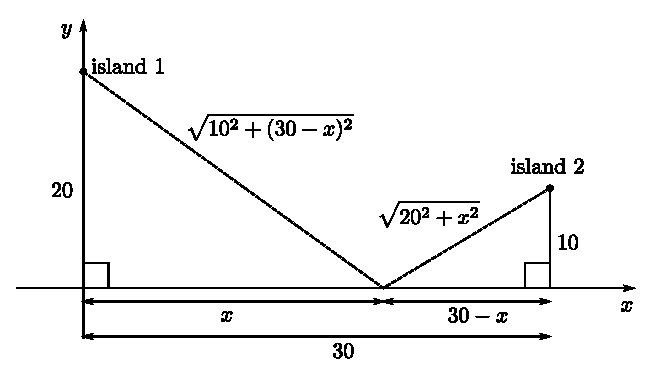
\includegraphics[scale=0.7]{img/island-set-up}
\caption{The set up of islands relative to the shore ($x$-axis).}
\label{fig:island-set-up}
\end{figure}

The total distance $D(x)$ to be travelled is given by the formula
\[D(x)=\sqrt{20^2+x^2}+\sqrt{10^2+(30-x)^2}.\]
On geometric grounds, we see that $0\le x \le 30$, and $D(x)$ is differentiable on this domain.
\begin{eqnarray*}
D'(x)&=&\frac{1}{2}(20^2+x^2)^{-\frac{1}{2}}\cdot2x+\frac{1}{2}\left(10^2+(30-x)^2\right)^{-\frac{1}{2}}2(30-x)\cdot-1\\
&=&\frac{x}{\sqrt{20^2+x^2}}-\frac{30-x}{\sqrt{(30-x)^2+10^2}}.
\end{eqnarray*}

To find the minimum distance we set $D'(x)=0$, so we have
\[\frac{x}{\sqrt{20^2+x^2}}=\frac{30-x}{\sqrt{(30-x)^2+10^2}}.\]
Squaring both sides we get
\[\frac{x^2}{20^2+x^2}=\frac{(30-x)^2}{(30-x)^2+10^2}\quad \implies \quad (x^2)[(30-x)^2+10^2]={(30-x)^2}(20^2+x^2) \]
Expanding the brackets we see
\[10^2x^2=20^2(30-x)^2.\]
Take the square root of both sides of the last equation gives
\[10x=\pm20(30-x).\]
Since $30-x\ge 0$ and $x\ge0$, the negative sign is not possible, so
\[10x=20(30-x)\quad \implies \quad x=20.\]
The only possible places where minimum can occur are
\[x=0,\quad x=20,\quad x=30,\]
where
\[D(0)=20+\sqrt{10^2+30^2}\approx 51.6,\]
\[D(20)=20\sqrt{2}+10\sqrt{2}=30\sqrt{2}\approx 42.4,\]
\[D(30)=\sqrt{20^2+30^2}+10\approx46.06.\]
So the minimum value does occur at $x=20$.

\begin{figure}[H]
\centering
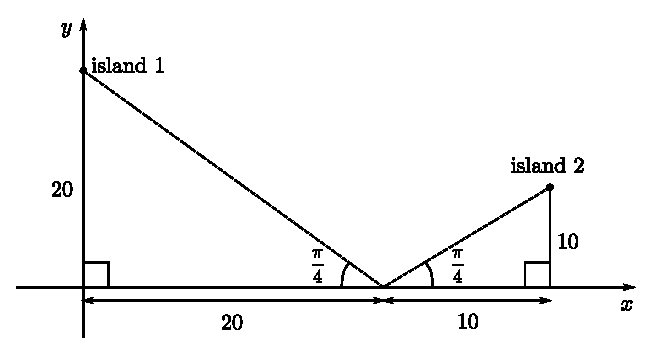
\includegraphics[scale=0.7]{img/island-opt-route}
\caption{Optimum route from island 1 to island 2, arriving and leaving shore at an angle of $\pi/4$ radians.}
\label{fig:island-opt-route}
\end{figure}

The optimal route is to leave the shore at the same angle of arrival.

Could we have deduced that this route was the shortest without calculus? Yes! We could have reflected island 2 in the shore line to obtain an imaginary island. Then it is easy to see that the shortest route from island 1 to the imaginary island is a straight line.

\begin{figure}[H]
\centering
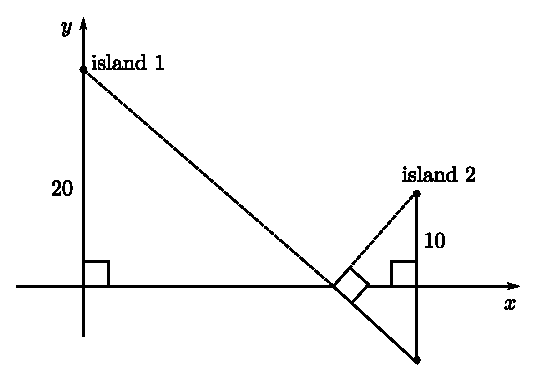
\includegraphics[scale=0.8]{img/island-alt-calc}
\caption{Sketch of alternative method of calculating shortest distance between the islands, using simple geometric properties, gaining same result.}
\label{fig:island-alt-calc}
\end{figure}

\end{example}

%MOTIVATING EXP EXAMPLE?
